\documentclass[a4paper, dvipsnames]{article}

\usepackage[T1]{fontenc}
\usepackage{geometry}
\geometry{
  left=2cm,
  right=2cm,
  top=4cm,
  bottom=4cm,
  bindingoffset=5mm
}

\usepackage{amssymb} 
\usepackage{amsmath}
\usepackage{amsthm}
\usepackage[utf8]{inputenc}
\usepackage[T1]{fontenc}
\usepackage{lmodern}
\usepackage{ngerman}
\usepackage{scrlayer-scrpage}
\usepackage{ulem}
\usepackage{xcolor}
\usepackage{graphicx}
\usepackage{listings}

\lstset{
language=Java,
aboveskip=3mm,
belowskip=3mm,
showstringspaces=false,
keywordstyle=\color{OliveGreen},
commentstyle=\color{gray},
breaklines=true,
breakatwhitespace=true,
tabsize=4
}

\pagestyle{scrheadings}

\ihead{Gruppe 10}
\chead{Logische Programmierung}
\ohead{\pagemark}

\setlength{\parindent}{0pt}


\begin{document}

{ \hspace{7,7cm}{\bfseries{Serie 1}}  {\hspace{6,0cm}{Gruppe 10}}\\

Adnan Alyousfi, 218205332, Informatik\\
Dirk Peglow, Informatik\\
Nils Henrik Seitz, 218205308, Informatik\\
Lorka Trad, Informatik\\
Nico Trebbin, 218204402, Informatik\\

\uline{\bfseries{Aufgabe 1}}\\
{\bfseries 1.C}\\
\begin{center}
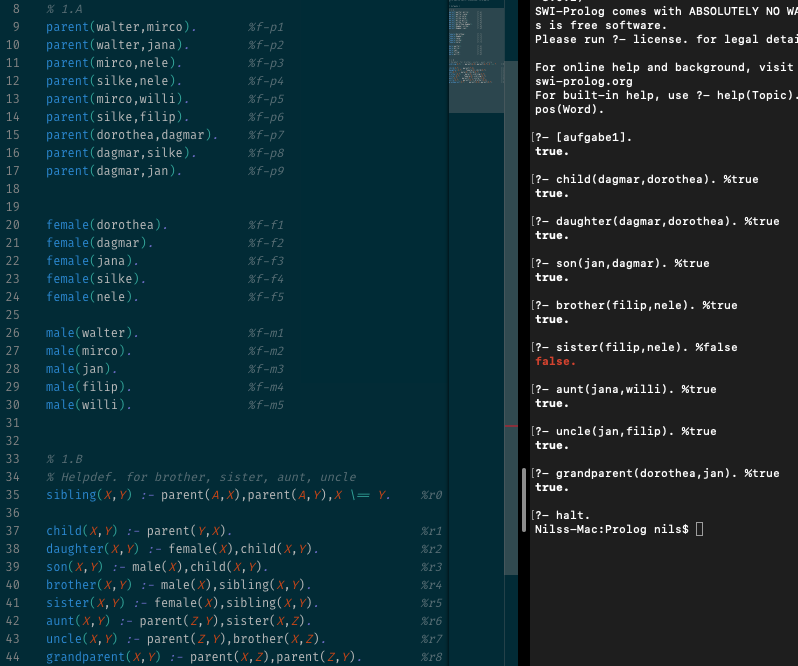
\includegraphics[width=0.5\textwidth]{Data/A1/C.png}
\end{center}


{\bfseries 1.D}\\

Der Übersichtlichkeit halber habe ich die Ableitungsbäume getrennt aufgeschrieben. Die einzelnen Ableitungsbäume werden der Reihe nach abgelaufen (d.h. Prolog durchläuft zuerst brother(X,Y) - Teil 1, und erst dann Teil 2)


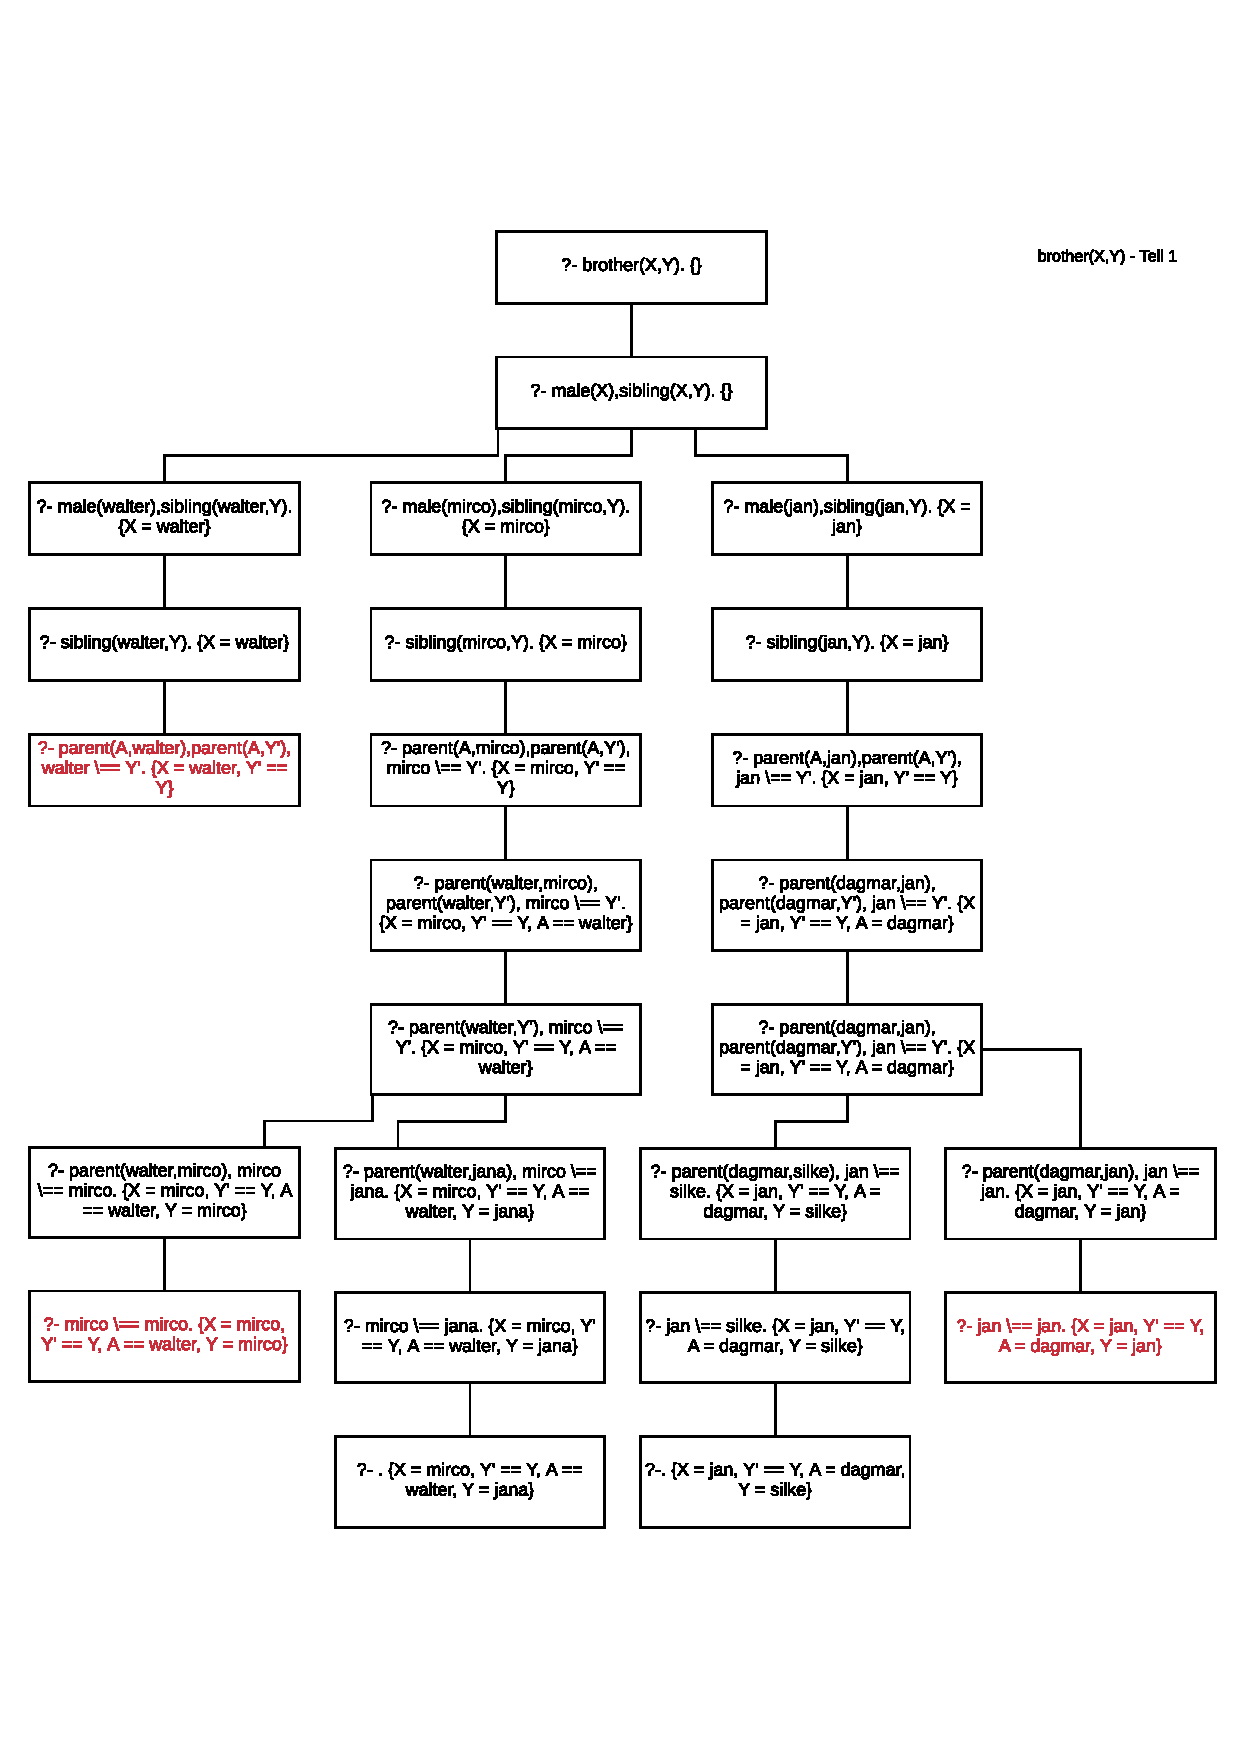
\includegraphics[width=1.0\textwidth]{Data/A1/1d1.pdf}
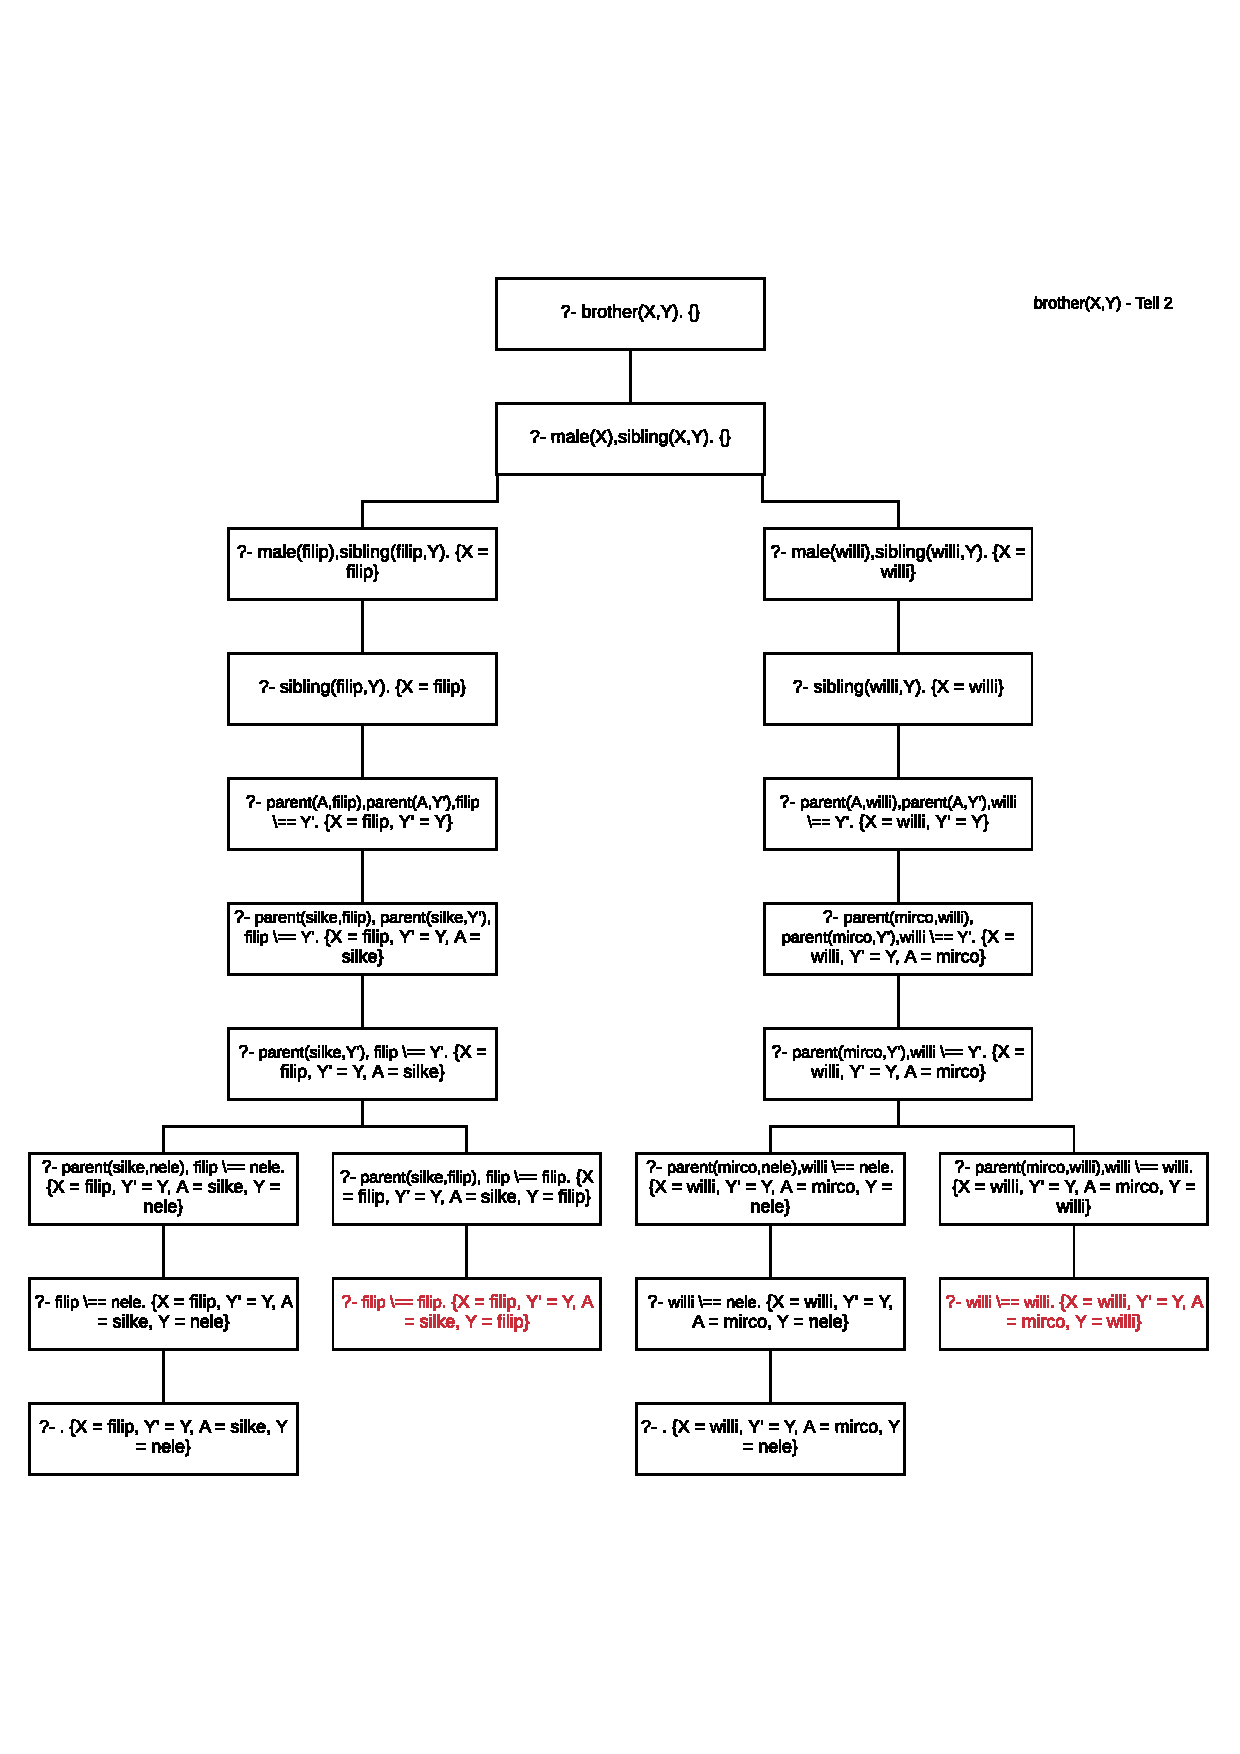
\includegraphics[width=1.0\textwidth]{Data/A1/1d2.pdf}
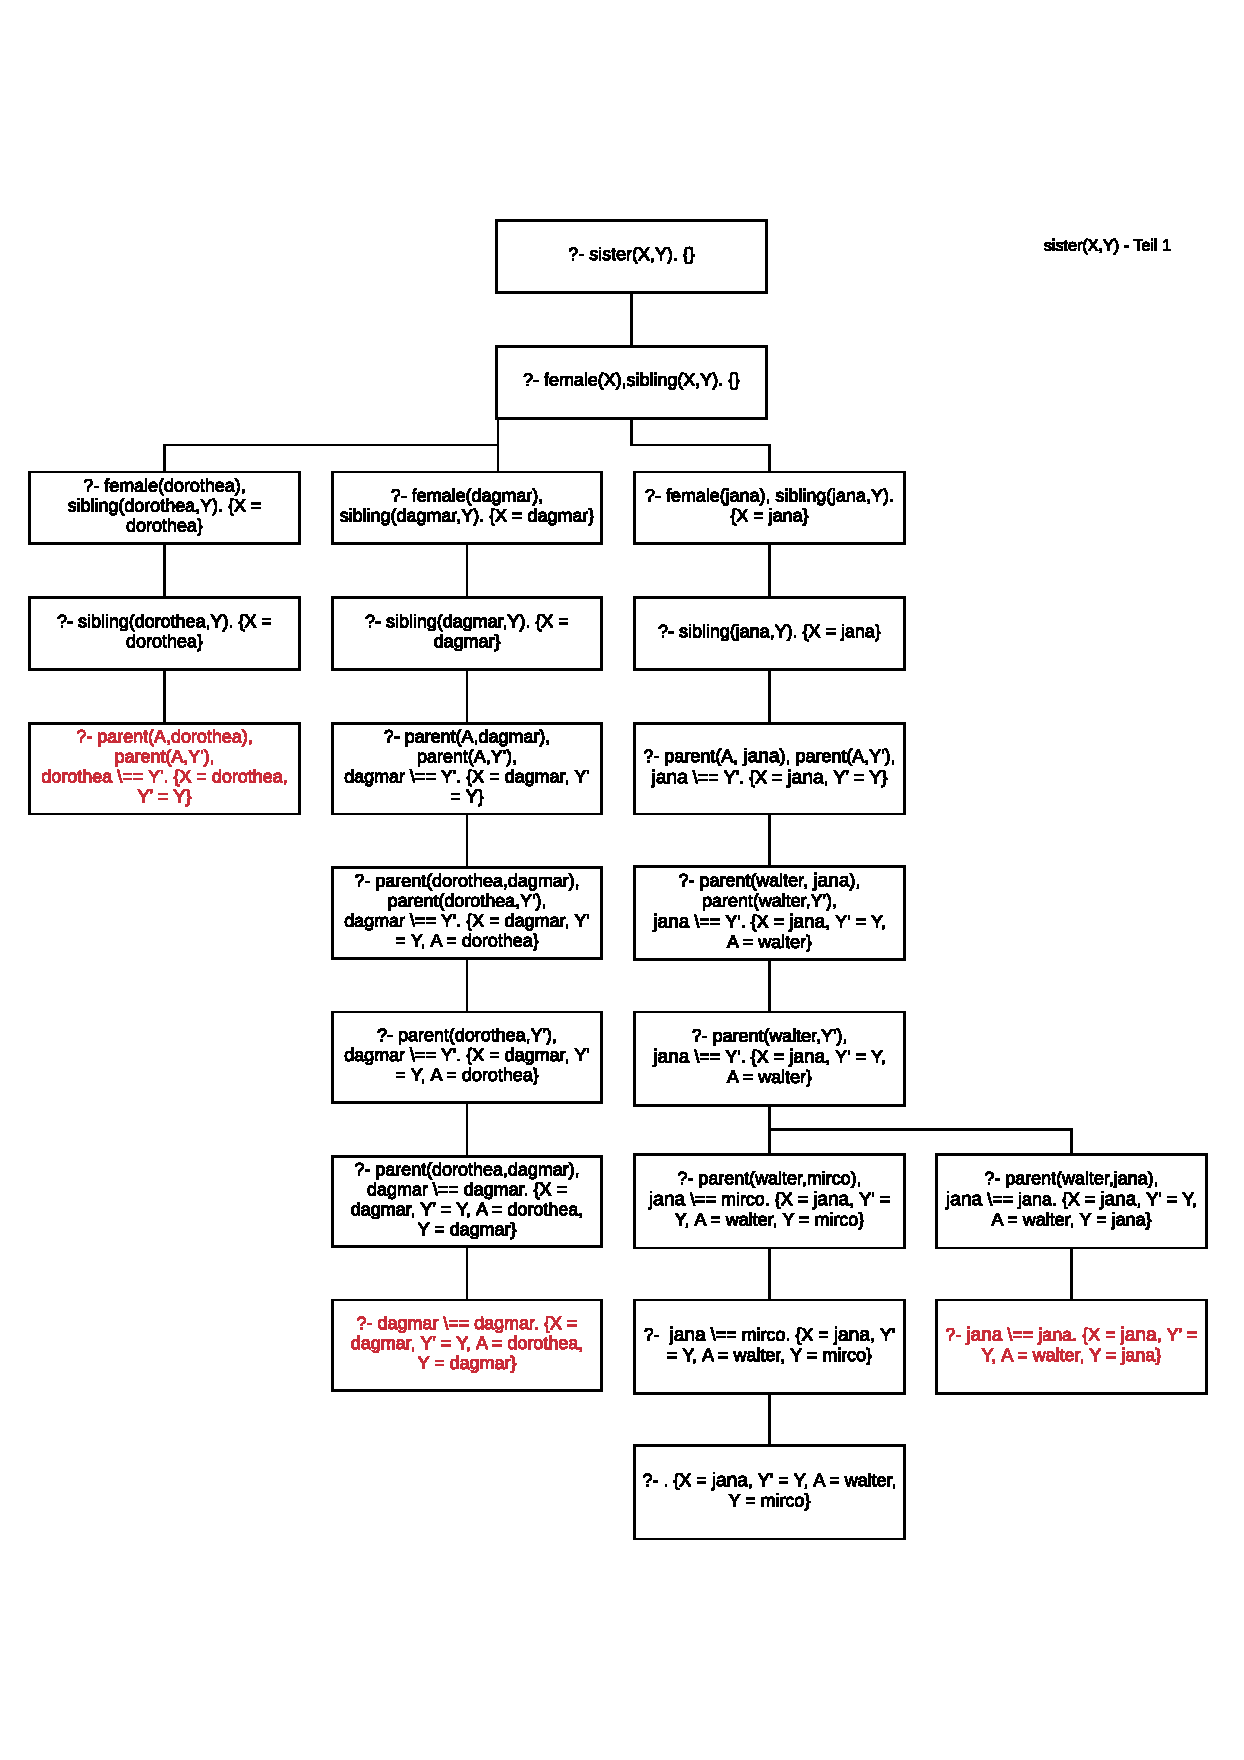
\includegraphics[width=1.0\textwidth]{Data/A1/1d3.pdf}
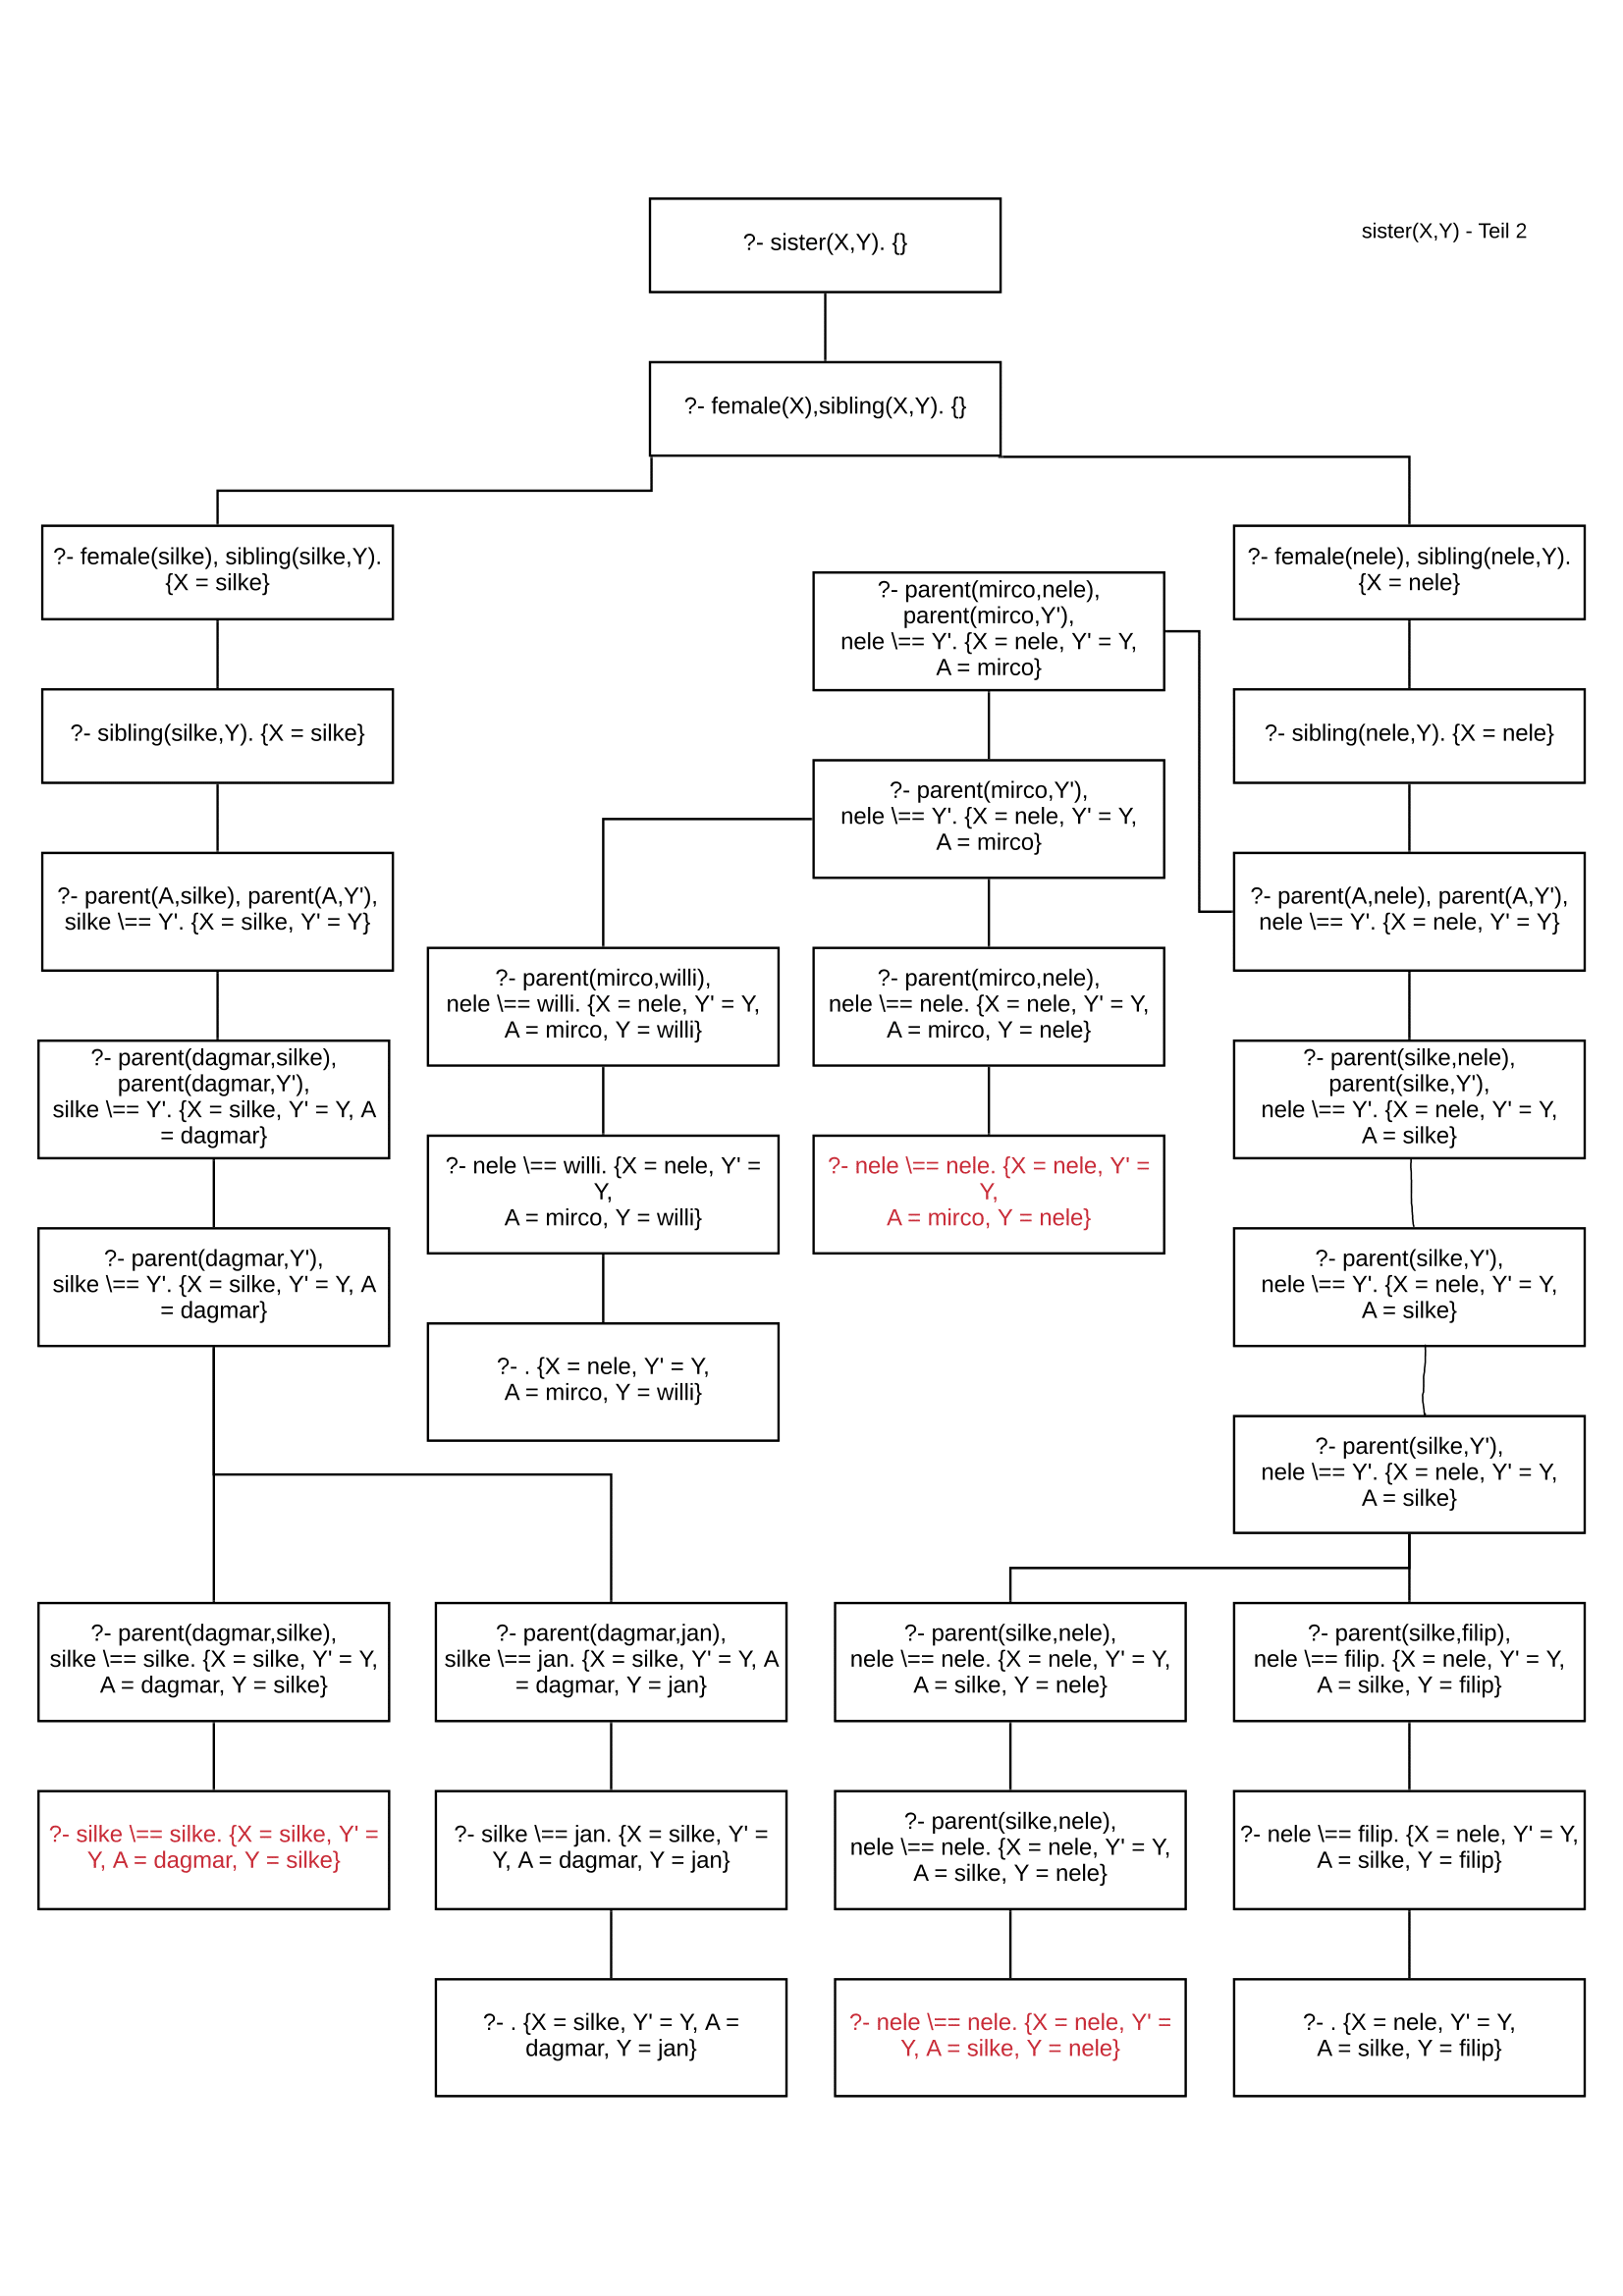
\includegraphics[width=1.0\textwidth]{Data/A1/1d4.png}
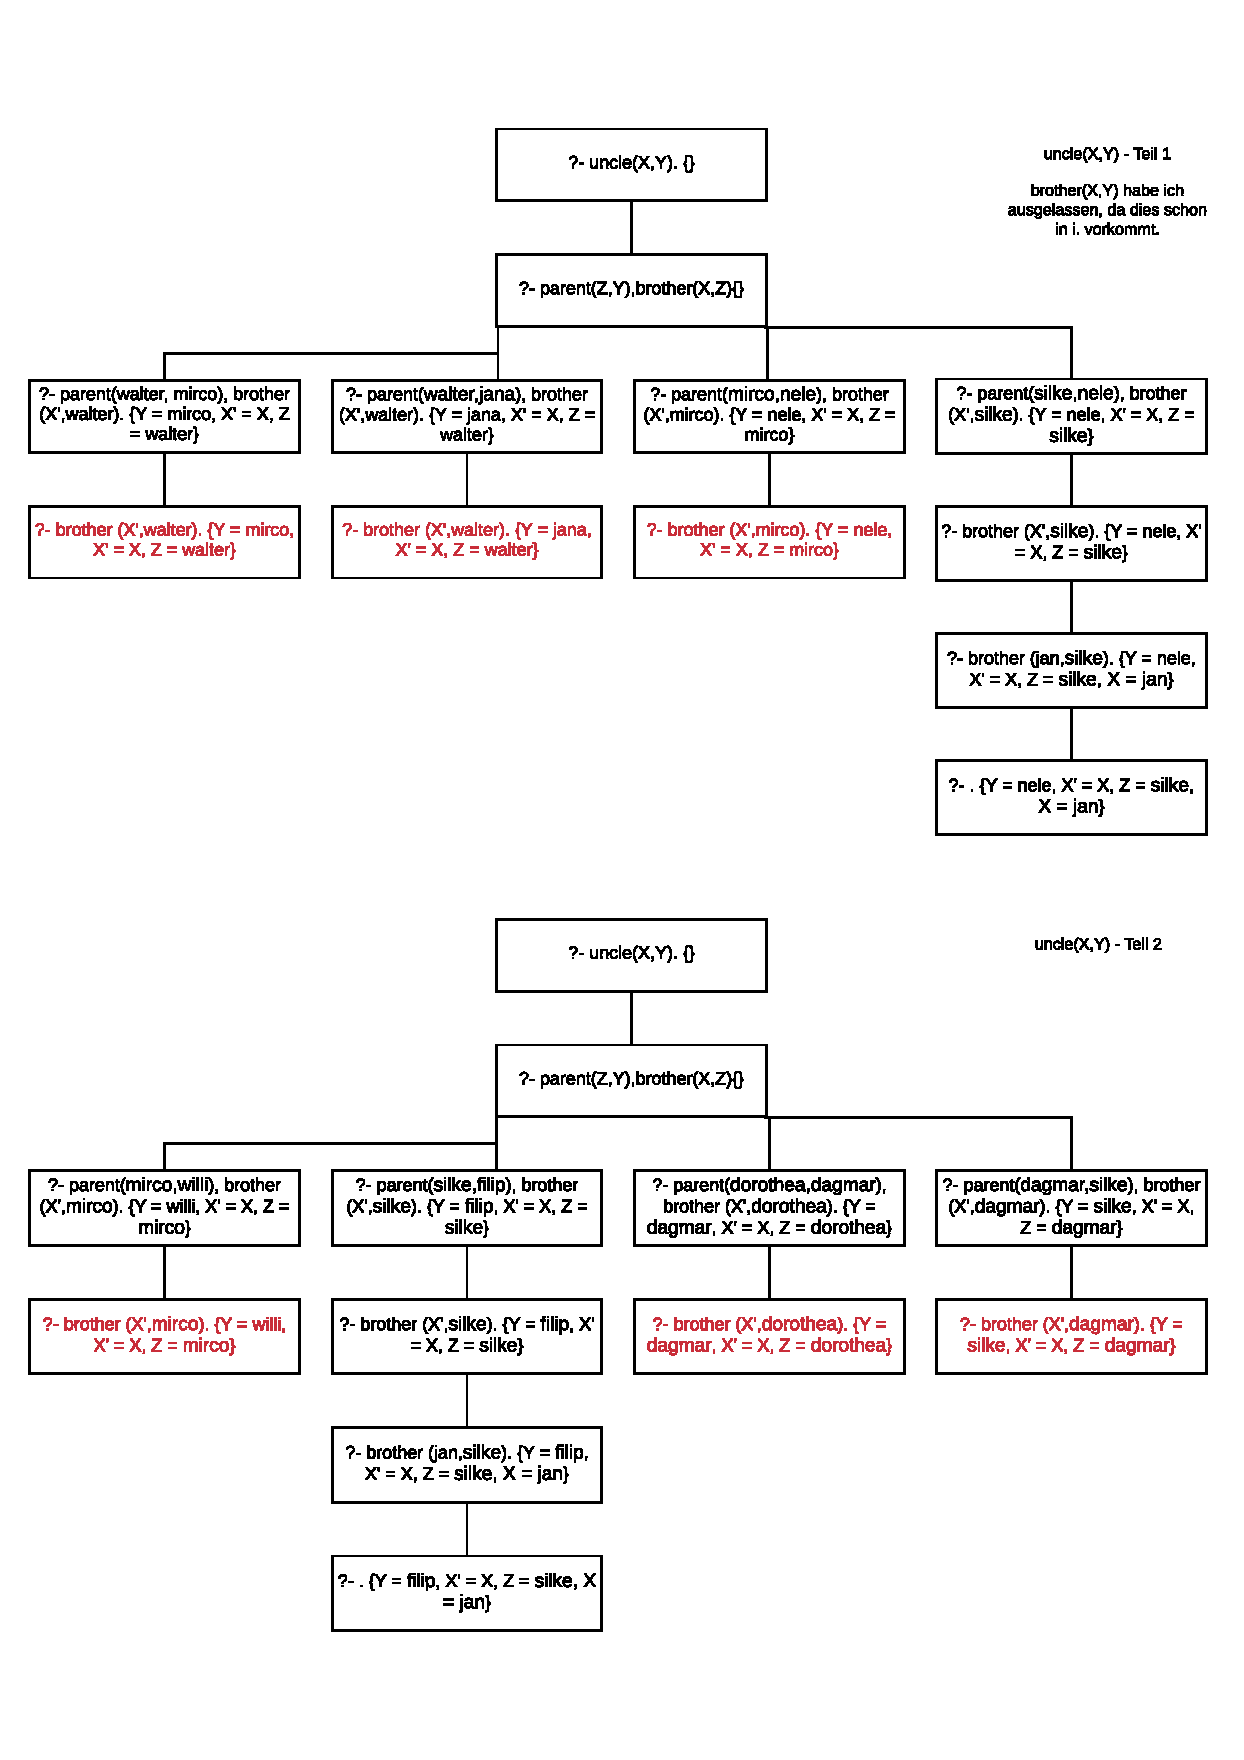
\includegraphics[width=1.0\textwidth]{Data/A1/1d5.pdf}
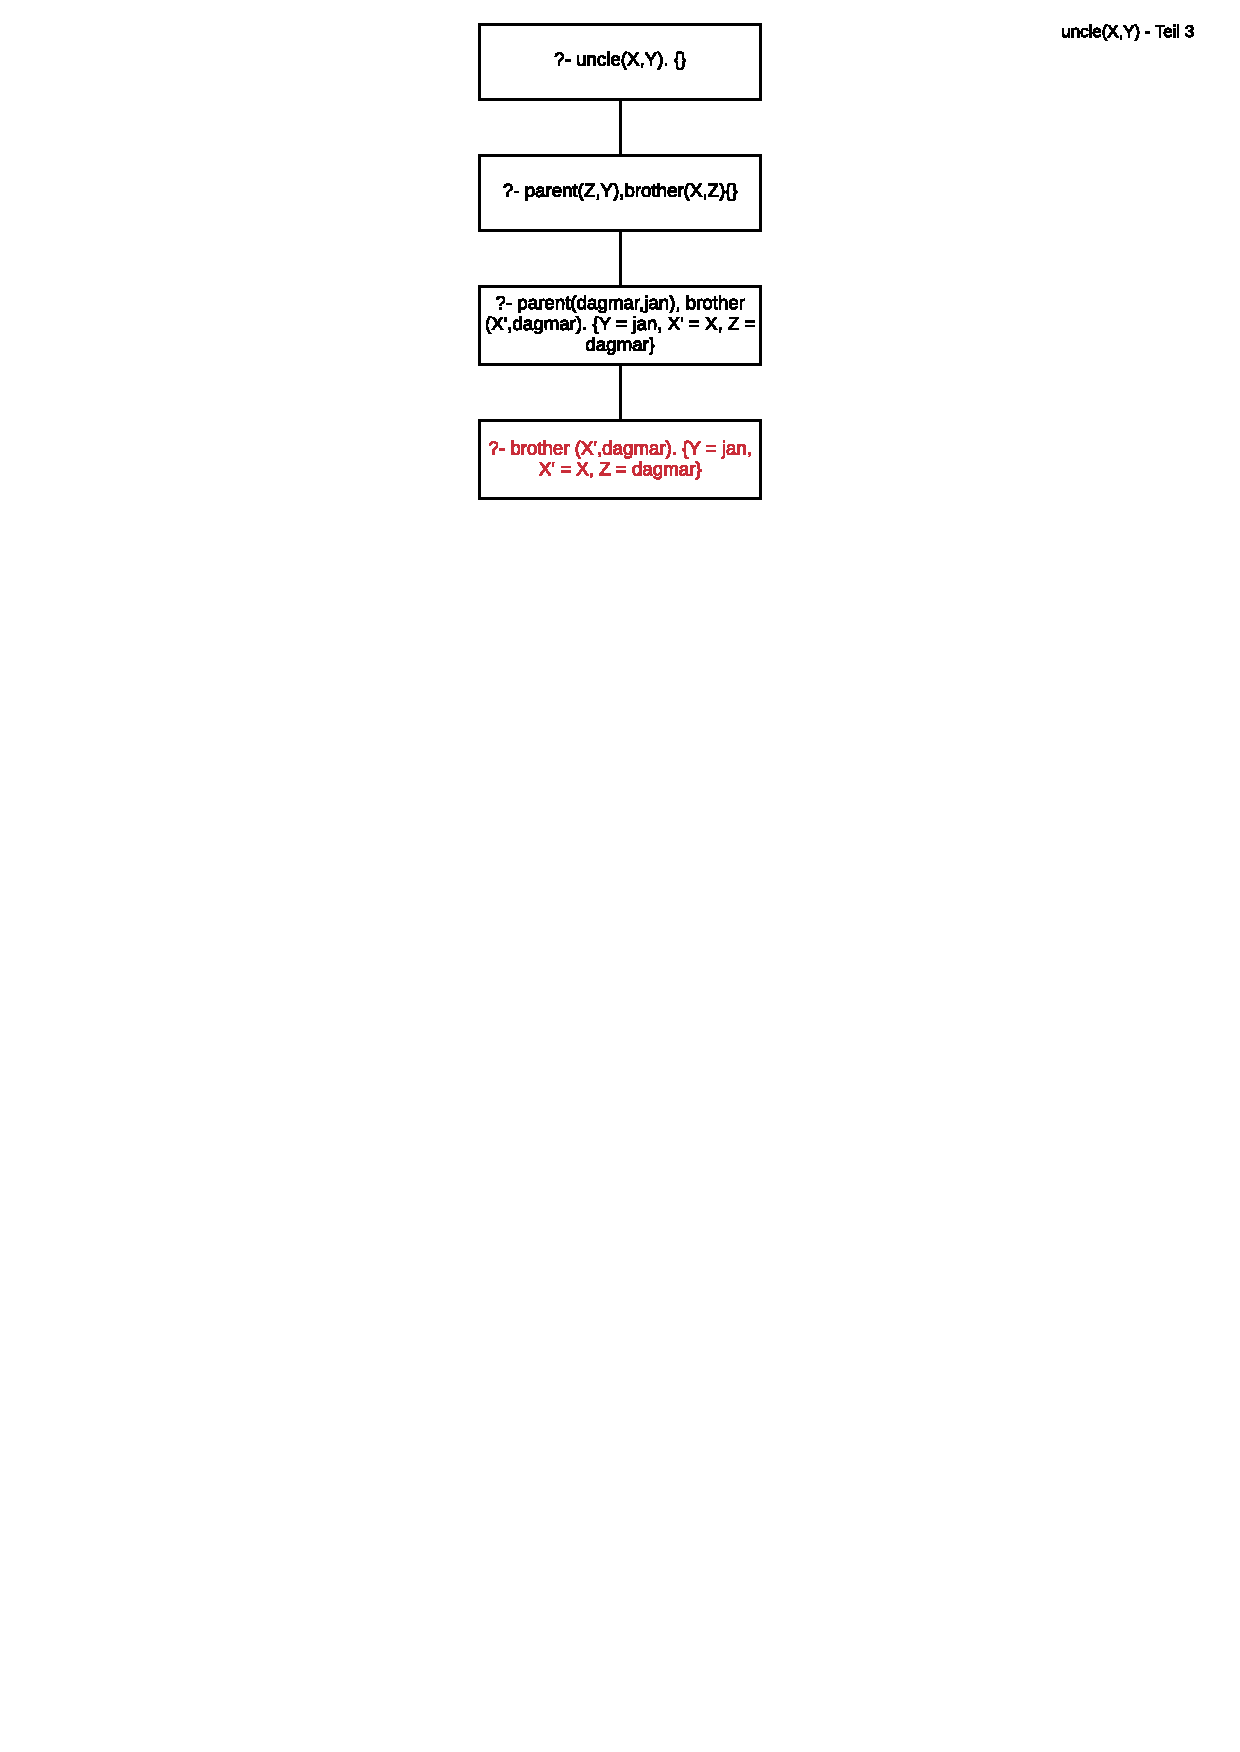
\includegraphics[width=1.0\textwidth]{Data/A1/1d52.pdf}
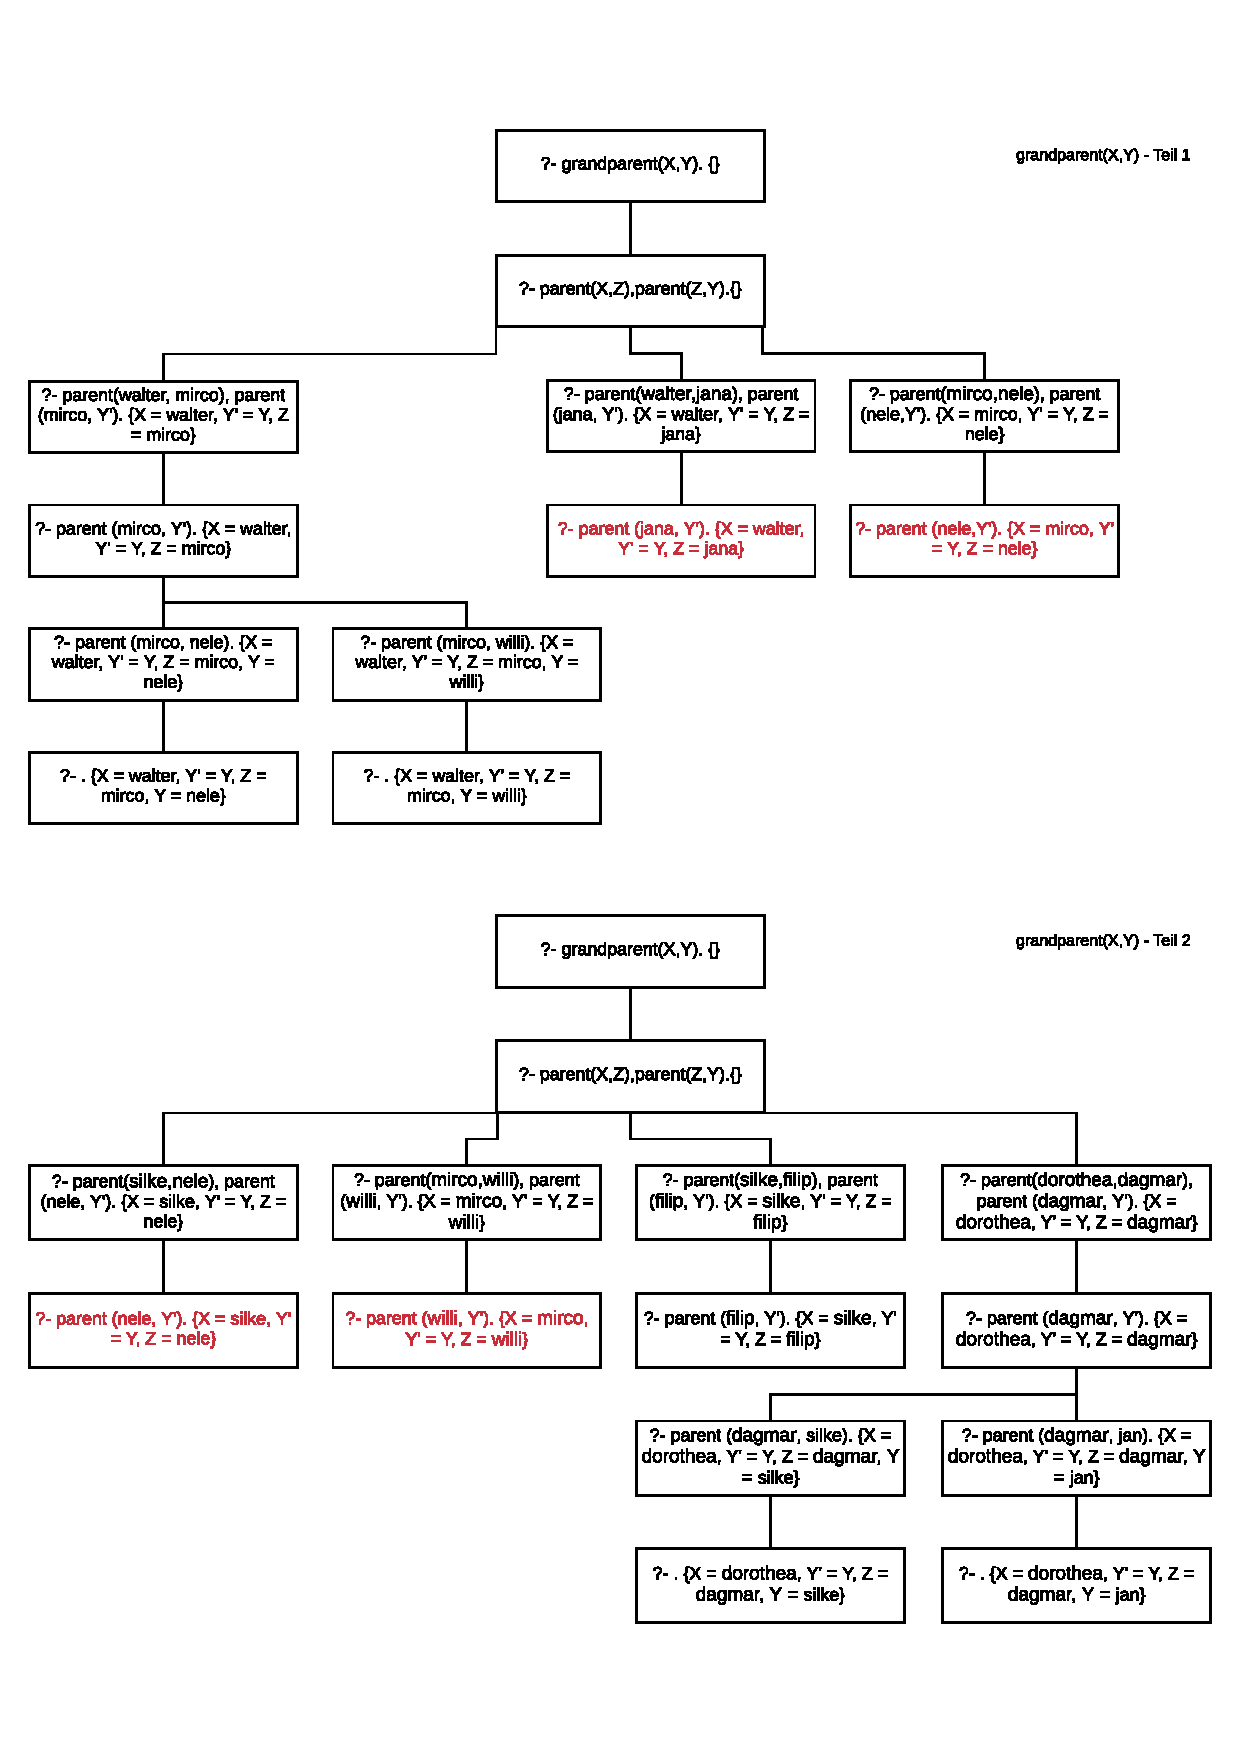
\includegraphics[width=1.0\textwidth]{Data/A1/1d6.pdf}
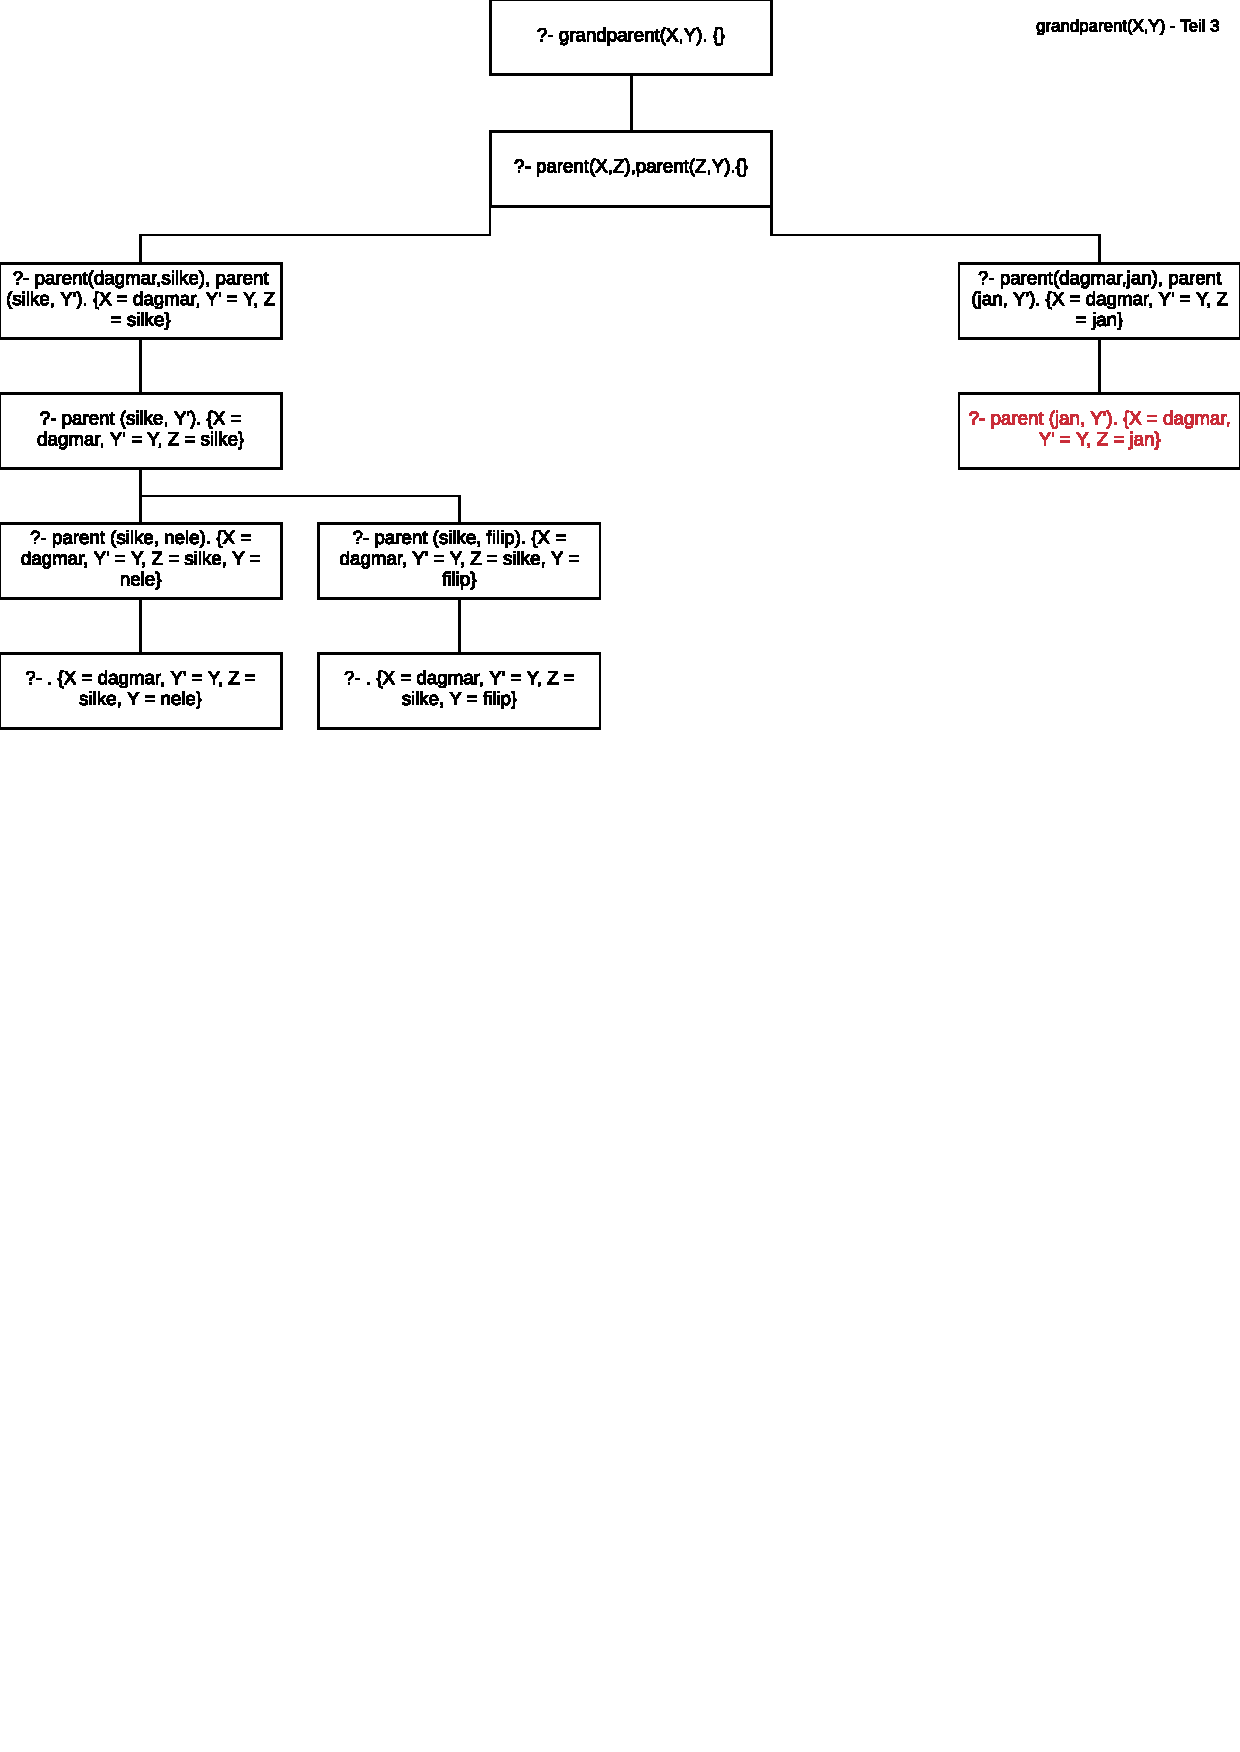
\includegraphics[width=1.0\textwidth]{Data/A1/1d7.pdf}


\uline{\bfseries{Aufgabe 2}}\\

{\bfseries 2.A}\\
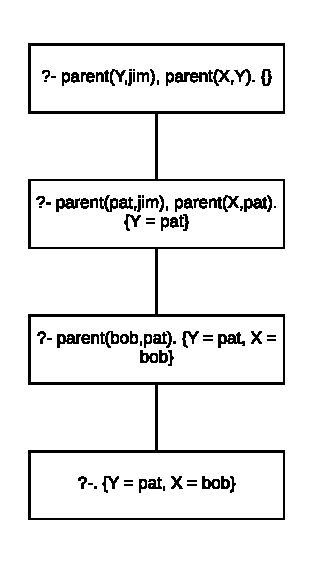
\includegraphics[width=0.3\textwidth]{Data/A2/a.pdf} \\

{\bfseries 2.B}\\
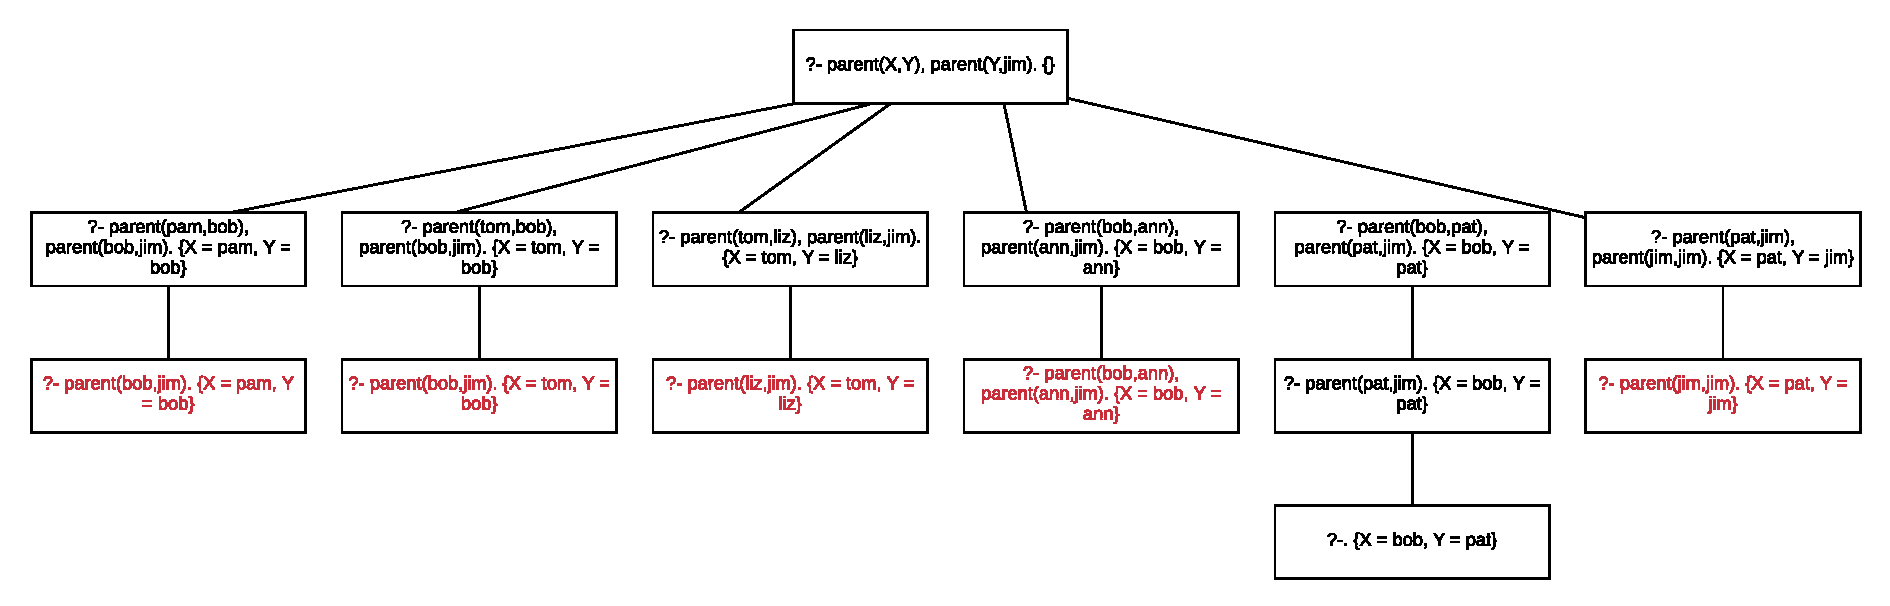
\includegraphics[width=1.0\textwidth]{Data/A2/b.pdf} \\

\uline{\bfseries{Aufgabe 4}}\\

{\bfseries 4.A}\\

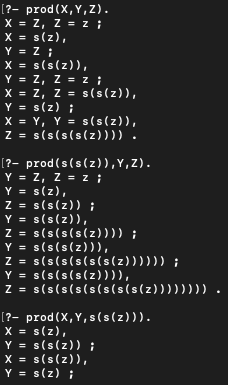
\includegraphics[width=0.4\textwidth]{Data/A4/4a.png} \\

{\bfseries Fehler: }\\

iii.) Prolog versucht alle möglichen Lösungen zu finden, in denen $X \cdot Y$ = 2 ist. Aufgrund fehlender Abbruchbedingung testet Prolog dieses Ergebnis auch mit $X,Y \geq 2$. Prolog versucht also alle Möglichkeiten durchzutesten, was zu einer Endlosschleife führt.
\end{document}
